\documentclass[11pt,a4paper]{article}

% ── Paquetes ──────────────────────────────────────────────────────────
\usepackage[utf8]{inputenc}
\usepackage[T1]{fontenc}
\usepackage[spanish]{babel}
\usepackage{geometry}
\usepackage{graphicx}
\usepackage{booktabs}
\usepackage{amsmath}
\usepackage{hyperref}
\usepackage{xcolor}
\usepackage{enumitem}
\usepackage{caption}
\usepackage{float}
\usepackage{fancyhdr}
\usepackage{parskip}
\usepackage{colortbl}

\geometry{top=2.5cm, bottom=2.5cm, left=2.5cm, right=2.5cm}

\definecolor{darkblue}{RGB}{0,51,102}
\definecolor{lightgray}{RGB}{240,240,240}

\hypersetup{colorlinks=true, linkcolor=darkblue, urlcolor=darkblue}

\setlist{itemsep=2pt, parsep=0pt}
\captionsetup{font=small, labelfont=bf, skip=6pt}

\pagestyle{fancy}
\fancyhf{}
\fancyhead[L]{\small Machine Learning II --- Práctica Final}
\fancyhead[R]{\small\thepage}
\renewcommand{\headrulewidth}{0.4pt}

\begin{document}

% ── Encabezado ────────────────────────────────────────────────────────
\begin{center}
    {\LARGE\bfseries Clasificador de Escenas Inmobiliarias}\\[4pt]
    {\large Transfer Learning y Ensemble con ConvNeXt y Swin Transformer}\\[12pt]
    {\normalsize
    Josep Maria Moyano Font \quad Carmen Miralles Gómez\\[2pt]
    Víctor del Águila Angulo \quad Ignacio Rojas Valenzuela}\\[8pt]
    {\small Machine Learning II --- Universidad Pontificia Comillas --- Abril 2026}
\end{center}
\vspace{6pt}
\hrule
\vspace{12pt}


% ══════════════════════════════════════════════════════════════════════
\section{Contexto de Negocio}
% ══════════════════════════════════════════════════════════════════════

Los portales inmobiliarios manejan cantidades enormes de fotografías de propiedades que suben tanto particulares como agencias. Hoy en día, etiquetar manualmente cada imagen según el tipo de estancia (dormitorio, cocina, salón\ldots) resulta caro, inconsistente y no escala bien. Nos planteamos resolver este problema construyendo un sistema que clasifique automáticamente imágenes de inmuebles en \textbf{15 categorías de escena}.

¿Qué valor aporta esto al negocio?
\begin{itemize}
    \item \textbf{Mejor experiencia de usuario}: los compradores pueden filtrar por tipo de estancia, las galerías se ordenan de forma coherente y se detectan imágenes mal categorizadas.
    \item \textbf{Ahorro en costes}: se elimina la revisión manual (estimamos unos 0.5\,s por imagen $\times$ millones de anuncios).
    \item \textbf{Datos más ricos}: se generan metadatos automáticos que alimentan sistemas de recomendación y valoración.
\end{itemize}

En cuanto a restricciones operativas, necesitamos una latencia de inferencia por debajo de 500\,ms por imagen, que el sistema funcione en una GPU de gama media (8\,GB de VRAM) y que sea accesible vía API REST para integrarse fácilmente con el backend de cualquier portal.


% ══════════════════════════════════════════════════════════════════════
\section{Arquitectura del Sistema}
% ══════════════════════════════════════════════════════════════════════

Hemos diseñado una arquitectura con tres capas bien diferenciadas:

\begin{enumerate}
    \item \textbf{Backend (FastAPI)}: un servicio de inferencia con endpoint \texttt{POST /predict} que recibe una imagen (JPEG, PNG o WebP, máx.\ 10\,MB), la preprocesa (resize, center crop, normalización ImageNet), la pasa por el modelo en GPU y devuelve la clase predicha, la confianza y la distribución de probabilidades sobre las 15 clases. También tiene endpoints de gestión: \texttt{GET /health} para comprobar el estado, \texttt{GET /models} para ver los modelos disponibles, \texttt{POST /models/select} para cambiar de modelo en caliente sin reiniciar el servidor, y documentación Swagger automática en \texttt{/docs}.

    \item \textbf{Frontend (Streamlit)}: una interfaz web con dos pestañas. En la primera se sube una imagen y se clasifica bajo demanda, mostrando las probabilidades de cada clase. En la segunda se activa la \textbf{webcam para clasificación en tiempo real}: cada fotograma se envía periódicamente al backend y la predicción se superpone directamente sobre el vídeo con un overlay de las top-5 clases. Además, incluye un selector dinámico de modelo en la barra lateral.

    \item \textbf{Experimentación (W\&B)}: todo el proceso de entrenamiento queda registrado en Weights \& Biases, incluyendo hiperparámetros, métricas por época, curvas de aprendizaje, artefactos de modelo y comparativas entre runs.
\end{enumerate}

\begin{figure}[H]
\centering
\fbox{\parbox{0.85\textwidth}{\centering\small
\texttt{Streamlit (puerto 8501)} $\longleftrightarrow$ \texttt{FastAPI (puerto 8001)} $\longleftrightarrow$ \texttt{PyTorch + CUDA}\\[4pt]
$\downarrow$\hspace{5cm}$\downarrow$\\[2pt]
\texttt{Webcam / Subida de imagen}\hspace{1.5cm}\texttt{Modelos timm en GPU}\\[4pt]
\texttt{W\&B Tracking} $\longleftrightarrow$ \texttt{Scripts de entrenamiento}
}}
\caption{Esquema general de la arquitectura del sistema.}
\label{fig:arch}
\end{figure}


% ══════════════════════════════════════════════════════════════════════
\section{Dataset}
% ══════════════════════════════════════════════════════════════════════

Trabajamos con el \texttt{scene\_dataset} proporcionado en el curso: \textbf{4,485 imágenes} repartidas en 15 clases de escena (Bedroom, Coast, Forest, Highway, Industrial, Inside City, Kitchen, Living Room, Mountain, Office, Open Country, Store, Street, Suburb y Tall Building).

\subsection{Proceso de Separación de Datos (Train / Validation / Test)}

\textbf{Estado inicial:} Las 4,485 imágenes se encontraban organizadas en \texttt{data/raw/} con una carpeta por cada clase (ej. \texttt{data/raw/Bedroom/}, \texttt{data/raw/Kitchen/}, etc.).

\textbf{Proceso de splitting:} Para garantizar que cada split (train, val, test) contuviera ejemplos balanceados de todas las clases, aplicamos la siguiente estrategia:

\begin{enumerate}
    \item Tomamos todas las imágenes de una clase (ej. los 216 dormitorios).
    \item Las barajeamos aleatoriamente usando una semilla fija (seed=42).
    \item Las dividimos en tres grupos secuenciales según los porcentajes:
    \begin{itemize}
        \item \textbf{Training}: primeras imágenes hasta el 70\% = 3,133 imágenes totales
        \item \textbf{Validation}: siguientes imágenes entre 70\% y 85\% = 668 imágenes totales
        \item \textbf{Test}: últimas imágenes desde 85\% = 684 imágenes totales
    \end{itemize}
    \item Repetimos este proceso para cada una de las 15 clases (garantizando que cada clase mantenga aproximadamente 70/15/15).
    \item Copiamos las imágenes a la estructura definitiva: \texttt{data/processed/train/}, \texttt{data/processed/val/} y \texttt{data/processed/test/}, cada una con subcarpetas por clase.
\end{enumerate}

\textbf{Resultado final:}
\begin{center}
\begin{tabular}{lcccc}
\toprule
\textbf{Split} & \textbf{Imágenes} & \textbf{\%} & \textbf{Uso en Pipeline} \\
\midrule
Training   & 3,133 & 69.9\% & Entrenamiento del modelo (con augmentación agresiva) \\
Validation & 668   & 14.9\% & Early stopping y selección de hiperparámetros \\
Test       & 684   & 15.2\% & Evaluación final del modelo (sin augmentación) \\
\midrule
\textbf{Total}    & 4,485 & 100\% & \\
\bottomrule
\end{tabular}
\end{center}

\textbf{Garantía de reproducibilidad:} Usamos \texttt{seed=42} en todas las operaciones de barajado. Esto asegura que ejecutando el código múltiples veces obtendremos exactamente la misma división de datos.

\textbf{Diagrama del flujo de datos:}

\begin{figure}[H]
\centering
\fbox{\parbox{0.9\textwidth}{\centering\small
\texttt{data/raw/} (4,485 imágenes)\\
\qquad Bedroom/ Coast/ Forest/ ... / Tall building/\\[8pt]
$\downarrow$ (split\_dataset.py con seed=42)\\[4pt]
\texttt{data/processed/}\\
\begin{tabular}{ccc}
train/ (70\%) & val/ (15\%) & test/ (15\%)\\
$\updownarrow$ Augmentación & $\updownarrow$ Determinista & $\updownarrow$ Determinista\\
3,133 imgs & 668 imgs & 684 imgs
\end{tabular}\\[4pt]
$\downarrow$ (get\_dataloaders.py)\\[4pt]
\texttt{DataLoader(shuffle=True, ...)} $\quad$ \texttt{DataLoader(shuffle=False, ...)}\\[2pt]
$\downarrow$\\
Entrenamiento (train) \quad Validación (val) \quad Evaluación (test)
}}
\caption{Flujo de separación de datos: desde raw hasta los dataloaders del entrenamiento.}
\label{fig:data-flow}
\end{figure}

\textbf{Desbalance de clases:} Existe un desbalance moderado (Kitchen tiene unas 210 imágenes frente a las 410 de Open Country, ratio $\approx$2$\times$), que gestionamos con augmentación agresiva y label smoothing en el entrenamiento.

\textbf{Nota sobre el balanceo por clase:} La proporción 70/15/15 se mantiene \textit{dentro de cada clase}, garantizando que todos los splits hereden el desbalance original del dataset (hay clases con 210 imágenes y otras con 410).



Durante el entrenamiento, cada split recibe transformaciones específicas:

\begin{itemize}
    \item \textbf{Training (3,133 imágenes):}
    \begin{itemize}
        \item RandomResizedCrop + RandomHorizontalFlip (flip horizontal aleatorio)
        \item ColorJitter (brillo, contraste, saturación, matiz) para simular variaciones de iluminación
        \item RandomRotation (hasta 15°) para robustez ante giros
        \item RandomPerspective (distorsión de perspectiva)
        \item RandomErasing (borrado aleatorio de regiones)
        \item Resize a 224×224 y normalización con stats de ImageNet
    \end{itemize}
    
    \item \textbf{Validation (668 imágenes):}
    \begin{itemize}
        \item Resize a 256×256 (escalado sin pérdida)
        \item CenterCrop a 224×224 (recorte determinista del centro)
        \item Normalización con stats de ImageNet
        \item \textbf{Sin augmentación:} las transformaciones son completamente deterministas
    \end{itemize}
    
    \item \textbf{Test (684 imágenes):}
    \begin{itemize}
        \item Idénticas a validation: Resize → CenterCrop → Normalización
        \item \textbf{Sin augmentación:} evaluación en condiciones de reproducibilidad total
    \end{itemize}
\end{itemize}

Esta estrategia de \textit{strong augmentation on train, weak on val/test} ayuda a regularizar el modelo y evitar sobreajuste.

\subsection{Uso de los Splits Durante el Entrenamiento}

Durante el loop de entrenamiento, cada split juega un papel específico y no se mezclan:

\begin{enumerate}
    \item \textbf{Época $n$:}
    \begin{itemize}
        \item Se itera sobre \textbf{todo el training set} (3,133 imágenes):
        \begin{itemize}
            \item Se aplican transformaciones agresivas
            \item Se calculan gradientes y se actualizan pesos
            \item Se registra train loss y train accuracy
        \end{itemize}
        \item Se evalúa el modelo sobre \textbf{todo el validation set} (668 imágenes):
        \begin{itemize}
            \item Sin gradientes (modo evaluación)
            \item Sin augmentación (transformaciones deterministas)
            \item Se registra val loss y val accuracy
        \end{itemize}
    \end{itemize}
    
    \item \textbf{Decision de Early Stopping:} Si val accuracy no mejora en 8 épocas, se detiene el entrenamiento y se carga el mejor checkpoint basado en val accuracy.
    
    \item \textbf{Tras finalizar el entrenamiento:}
    \begin{itemize}
        \item Se carga el \textbf{best model} (el guardado con mayor val accuracy)
        \item Se evalúa sobre el \textbf{test set} (684 imágenes) por primera vez
        \item Test accuracy es la métrica final de generalización (nunca se usa en el loop de training)
    \end{itemize}
\end{enumerate}

\textbf{Por qué esta separación es crítica:}
\begin{itemize}
    \item \textbf{Training} proporciona la señal para aprender (con augmentación).
    \item \textbf{Validation} mide la generalización sin contaminar los pesos (es el ``árbitro'' para seleccionar el mejor modelo).
    \item \textbf{Test} es completamente independiente y untouched: es la evaluación honesta del rendimiento del modelo.
\end{itemize}

Cualquier fuga de información entre estos conjuntos comprometería la credibilidad de nuestros resultados.

\begin{figure}[H]
\centering
\fbox{\parbox{0.95\textwidth}{\centering\small
\textbf{Flujo temporal del entrenamiento:}\\[8pt]
\begin{tabular}{cccc}
\textbf{Época 1} & $\cdots$ & \textbf{Época 20} & \textbf{Época 25 (última)}\\
\hline
\scriptsize
\begin{tabular}{c}
Train: 3,133 \\
(actualizar pesos)\\
$\downarrow$\\
Val: 668\\
(medir, no gradientes)\\
$\rightarrow$\\
val\_acc = 87.1\%\\
$\checkmark$ best
\end{tabular}
&
$\vdots$
&
\scriptsize
\begin{tabular}{c}
Train: 3,133 \\
(actualizar pesos)\\
$\downarrow$\\
Val: 668\\
(medir, no gradientes)\\
$\rightarrow$\\
val\_acc = 88.9\%\\
(sin mejora $\times$8)\\
\textbf{STOP}
\end{tabular}
&
\scriptsize
\begin{tabular}{c}
Cargar best model\\
$\downarrow$\\
Test: 684\\
(primera vez,\\
EVAL FINAL)\\
$\rightarrow$\\
test\_acc = 87.4\%\\
\end{tabular}
\end{tabular}\\[8pt]
\end{tabular}\\[4pt]
Resultado: \textbf{Test Accuracy 87.4\%} (métrica honesta de generalización)
}}
\caption{Línea de tiempo del entrenamiento mostrando cómo cada split es usado exactamente una vez por época (excepto test, que se usa solo al final).}
\label{fig:training-timeline}
\end{figure}

\textbf{Resumen de la estrategia de separación:}

El enfoque de tres conjuntos (train/val/test) es el estándar en machine learning porque:
\begin{itemize}
    \item \textbf{Training} permite al modelo aprender patrones comunes en los datos.
    \item \textbf{Validation} actúa como mecanismo de control para evitar sobreajuste y para seleccionar el mejor estado del modelo.
    \item \textbf{Test} garantiza una evaluación final objetiva que nunca ha influido en la optimización.
\end{itemize}

En nuestro caso: \textbf{4,485 imágenes} $\to$ \textbf{split 70/15/15} $\to$ \textbf{3,133 train + 668 val + 684 test}. Cada imagen de entrada aparece exactamente en uno de los tres conjuntos. La augmentación de datos ocurre únicamente en training para no contaminar las métricas de validación y test. El resultado es un modelo que alcanza una \textbf{test accuracy de 87.4\%}, que es la métrica final y confiable de su capacidad de generalización.


% ══════════════════════════════════════════════════════════════════════
\section{Enfoque de Modelado}
% ══════════════════════════════════════════════════════════════════════

\subsection{Estrategia de Transfer Learning}

Nuestra estrategia se basa en hacer \textit{fine-tuning completo} de backbones preentrenados en ImageNet-22k (14.2 millones de imágenes, 21,843 clases) y después afinados en ImageNet-1k. Esto nos da representaciones mucho más ricas que usar solo ImageNet-1k. Todos los parámetros del backbone son entrenables, pero usamos \textbf{learning rates discriminativos}: al backbone le asignamos un lr muy bajo (entre 1e-5 y 2e-5) para no destruir las features aprendidas, y al head de clasificación le damos 50$\times$ más (5e-4 a 1e-3), ya que se inicializa desde cero.

\subsection{Cabeza de Clasificación}

Sustituimos el clasificador original del backbone por un MLP de 3 capas lineales que diseñamos nosotros:

\begin{center}
\small
\texttt{BN(768) $\to$ Drop(0.4) $\to$ Linear(768,512) $\to$ GELU $\to$ Drop(0.2) $\to$ Linear(512,256) $\to$ GELU $\to$ Drop(0.12) $\to$ Linear(256,15)}
\end{center}

El dropout va descendiendo conforme nos acercamos a la salida: más regularización cerca de las features generales del backbone y menos cerca de la predicción final. Observamos que esto mejora la calibración del modelo.

\subsection{Técnicas de Regularización}

Además de la augmentación de datos estándar (RandomResizedCrop, flips, ColorJitter, rotación, perspectiva y RandomErasing), aplicamos:

\begin{itemize}
    \item \textbf{Mixup} ($\alpha=0.3$): mezcla lineal de pares de imágenes y sus etiquetas.
    \item \textbf{CutMix} ($\alpha=1.0$): recorta una región de una imagen y la pega sobre otra, ajustando las etiquetas proporcionalmente.
    \item \textbf{Label Smoothing} ($\epsilon=0.1$): suaviza los targets de $[0,1]$ a $[0.007, 0.933]$ para evitar sobreconfianza.
\end{itemize}

\subsection{Configuración del Entrenamiento}

Usamos \textbf{AdamW} con weight decay de 0.05, \textbf{warmup lineal} de 3 épocas seguido de \textbf{cosine annealing}, \textbf{mixed precision} (AMP) para acelerar y ahorrar VRAM, y \textbf{gradient clipping} (max\_norm=1.0). El early stopping salta tras 8 épocas sin mejora superior al 0.15\% en val accuracy, con un mínimo de 8--10 épocas para dejar al modelo estabilizarse.

\subsection{Modelos Finales}

Tras toda la experimentación, nos quedamos con tres modelos:

\begin{enumerate}
    \item \textbf{ConvNeXt-Small} (288px): CNN modernizada de 49.9M parámetros, 36 bloques. Nuestro mejor modelo individual.
    \item \textbf{ConvNeXt-Tiny} (288px): versión más compacta, 28.4M parámetros, 18 bloques.
    \item \textbf{Swin Transformer Tiny} (224px): Vision Transformer con atención por ventanas, 28.0M parámetros.
\end{enumerate}


% ══════════════════════════════════════════════════════════════════════
\section{Proceso de Experimentación con W\&B}
% ══════════════════════════════════════════════════════════════════════

\subsection{Fases del Proceso}

Nuestra experimentación fue iterativa y pasó por cuatro fases, todas registradas en Weights \& Biases:

\textbf{Fase 1 --- Baselines en CPU.} Empezamos con 3 runs de EfficientNet-B0 a 224px para tener una referencia. Obtuvimos entre un 84\% y un 87\% de val accuracy con augmentación media.

\textbf{Fase 2 --- Fine-tuning completo en GPU.} Pasamos a GPU y probamos EfficientNet-B0 con AdamW, label smoothing y AMP. Subimos a un 94.46\% en val, lo que nos confirmó que descongelar todo el backbone era fundamental.

\textbf{Fase 3 --- Backbones avanzados.} Aquí dimos el salto de calidad: probamos ConvNeXt-Tiny (288px), EfficientNet-B4 (380px), Swin-Tiny (224px), ConvNeXt-Small (288px), DenseNet-161 (288px) y EfficientNet-B0 (288px) con todas las técnicas avanzadas. ConvNeXt-Tiny fue el primero en superar el 97\% en validación (97.31\%).

\textbf{Fase 4 --- Ensemble.} Entrenamos Swin-Tiny y ConvNeXt-Small, y luego evaluamos todas las combinaciones posibles de ensemble con Test-Time Augmentation (TTA).

\subsection{Sweep de Hiperparámetros}

Configuramos un \textbf{sweep bayesiano} en W\&B explorando 12 hiperparámetros: backbone, learning rate (log-uniform entre 1e-5 y 1e-2), dropout (0.2--0.5), optimizador (Adam, AdamW, SGD), weight decay, freeze/unfreeze del backbone, batch size (16--64), scheduler (cosine, step, none), nivel de augmentación, dimensión del head (128--512) y número de capas del head (1--2).

Las conclusiones del sweep fueron claras: AdamW es el mejor optimizador, la augmentación heavy da los mejores resultados, cosine annealing supera a step scheduling, y los heads de 512 dimensiones con 2 capas rinden más que los de 128 o 256 con 1 capa.

\subsection{Criterio de Selección}

Para elegir el modelo final, nos fijamos principalmente en la \textbf{accuracy en test con TTA}, usando macro-F1 como métrica secundaria (importante dado el desbalance entre clases). El ensemble de ConvNeXt-Tiny + ConvNeXt-Small resultó ser la mejor combinación, con un 97.37\% de accuracy y 97.62\% de F1.

\begin{figure}[H]
\centering
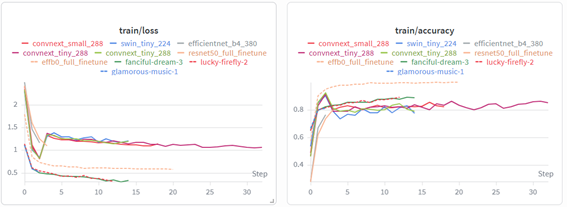
\includegraphics[width=0.95\textwidth]{capturas/Train_todos_modelos.png}
\caption{Curvas de entrenamiento de todos los modelos en W\&B. Los ConvNeXt convergen mucho más rápido que los baselines de EfficientNet-B0.}
\label{fig:train_all}
\end{figure}

\begin{figure}[H]
\centering
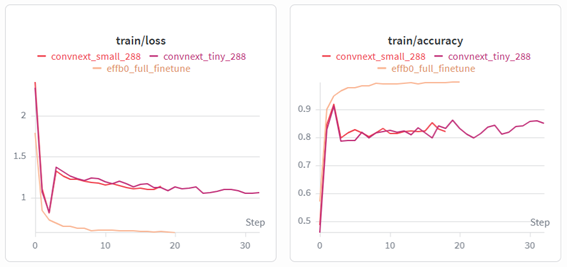
\includegraphics[width=0.95\textwidth]{capturas/Train_3_mejores.png}
\caption{Loss y accuracy de entrenamiento de los 3 mejores modelos. La accuracy de train aparece baja ($\sim$82\%) porque se calcula sobre imágenes mezcladas por Mixup/CutMix, no indica underfitting.}
\label{fig:train_top3}
\end{figure}

\begin{figure}[H]
\centering
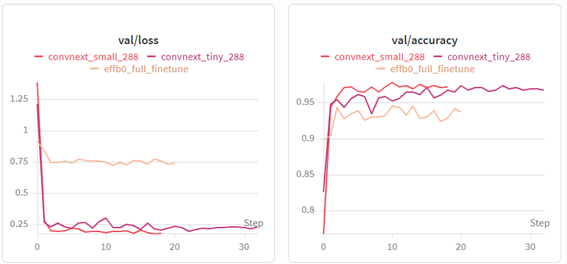
\includegraphics[width=0.95\textwidth]{capturas/Test_3_mejores.png}
\caption{Loss y accuracy de validación de los 3 mejores modelos. ConvNeXt-Small alcanza su pico (97.75\%) en la época 11.}
\label{fig:val_top3}
\end{figure}


% ══════════════════════════════════════════════════════════════════════
\section{Métricas de Rendimiento por Clase}
% ══════════════════════════════════════════════════════════════════════

En la Tabla~\ref{tab:perclass} mostramos las métricas detalladas por clase de nuestro ensemble final (ConvNeXt-Tiny + ConvNeXt-Small con TTA) evaluado sobre las 684 imágenes de test.

\begin{table}[H]
\centering
\caption{Métricas por clase del ensemble final en el conjunto de test.}
\label{tab:perclass}
\begin{tabular}{lcccc}
\toprule
\textbf{Clase} & \textbf{Precision} & \textbf{Recall} & \textbf{F1-Score} & \textbf{Soporte} \\
\midrule
Bedroom        & 1.00 & 1.00 & 1.00 & 33 \\
Coast          & 0.96 & 0.95 & 0.95 & 55 \\
Forest         & 0.96 & 1.00 & 0.98 & 50 \\
Highway        & 0.97 & 0.97 & 0.97 & 39 \\
Industrial     & 0.98 & 1.00 & 0.99 & 48 \\
Inside City    & 1.00 & 0.91 & 0.96 & 47 \\
Kitchen        & 1.00 & 0.94 & 0.97 & 32 \\
Living Room    & 0.98 & 1.00 & 0.99 & 44 \\
Mountain       & 1.00 & 0.95 & 0.97 & 57 \\
Office         & 1.00 & 1.00 & 1.00 & 33 \\
Open Country   & 0.91 & 0.94 & 0.92 & 62 \\
Store          & 0.98 & 1.00 & 0.99 & 48 \\
Street         & 0.94 & 1.00 & 0.97 & 45 \\
Suburb         & 1.00 & 1.00 & 1.00 & 37 \\
Tall Building  & 0.98 & 0.98 & 0.98 & 54 \\
\midrule
\textbf{Macro Avg} & \textbf{0.98} & \textbf{0.98} & \textbf{0.98} & \textbf{684} \\
\bottomrule
\end{tabular}
\end{table}

Las clases con F1 perfecto (Bedroom, Office, Suburb) son escenas con patrones visuales muy distintivos y fáciles de separar. La clase más complicada es Open Country (F1=0.92), que a veces se confunde con Coast y Mountain porque comparten paisajes naturales abiertos. Inside City pierde algo de recall (0.91) hacia Street, lo cual tiene sentido semántico.

Lo importante para el negocio es que las clases de interior ---Bedroom, Kitchen, Living Room, Office--- que son las más relevantes en un portal inmobiliario, alcanzan todas un F1~$\geq$~0.97, lo que consideramos suficiente para producción.

En la Tabla~\ref{tab:comparison} comparamos los modelos finales:

\begin{table}[H]
\centering
\caption{Comparativa de los modelos finales.}
\label{tab:comparison}
\begin{tabular}{lcccc}
\toprule
\textbf{Modelo} & \textbf{Parámetros} & \textbf{Val Acc} & \textbf{Test+TTA} & \textbf{Macro-F1} \\
\midrule
ConvNeXt-Small  & 49.9M & 97.75\% & 96.93\% & 96.66\% \\
ConvNeXt-Tiny   & 28.4M & 97.31\% & 96.05\% & 96.50\% \\
Swin-Tiny       & 28.0M & 96.41\% & 95.61\% & 95.96\% \\
\rowcolor{lightgray}
\textbf{Ensemble (T+S)} & \textbf{78.3M} & --- & \textbf{97.37\%} & \textbf{97.62\%} \\
\bottomrule
\end{tabular}
\end{table}


% ══════════════════════════════════════════════════════════════════════
\section{Documentación de la API}
% ══════════════════════════════════════════════════════════════════════

La API REST genera documentación OpenAPI/Swagger automáticamente, accesible en \texttt{/docs}. Estos son los endpoints:

\textbf{\texttt{POST /predict}} --- Clasifica una imagen.
\begin{itemize}
    \item \textbf{Input}: archivo de imagen vía multipart/form-data (JPEG, PNG o WebP, máx.\ 10\,MB).
    \item \textbf{Output (200)}: JSON con \texttt{model\_name}, \texttt{predicted\_class}, \texttt{confidence} (entre 0 y 1) y \texttt{probabilities} (diccionario con la probabilidad de cada una de las 15 clases).
    \item \textbf{Errores}: 400 si el tipo de archivo no es válido o la imagen está corrupta; 503 si no hay ningún modelo cargado.
\end{itemize}

\textbf{\texttt{GET /health}} --- Devuelve el estado del servicio: si el modelo está cargado, en qué dispositivo (CPU/CUDA), qué modelo está activo, su backbone y resolución.

\textbf{\texttt{GET /models}} --- Lista todos los modelos disponibles con sus métricas (val\_acc, test\_acc, test\_tta\_acc, macro\_f1) e indica cuál está activo.

\textbf{\texttt{POST /models/select}} --- Permite cambiar de modelo en caliente enviando \texttt{\{"name": "convnext\_small\_288"\}}. Carga el checkpoint correspondiente sin reiniciar el servidor.

Todos los endpoints usan validación con Pydantic, tienen CORS habilitado y siguen convenciones RESTful con códigos HTTP estándar.


% ══════════════════════════════════════════════════════════════════════
\section{Enlaces del Proyecto}
% ══════════════════════════════════════════════════════════════════════

\begin{itemize}
    \item \textbf{Repositorio Git}: \url{https://github.com/nachomgf/real-estate-classifier} (público, con instrucciones de setup en el README).
    \item \textbf{Proyecto W\&B}: \url{https://wandb.ai/202525416-universidad-pontificia-comillas/real-estate-classifier}
\end{itemize}

Se ha invitado a \texttt{agascon@comillas.edu} y \texttt{rkramer@comillas.edu} al workspace de W\&B.


% ══════════════════════════════════════════════════════════════════════
\section{Instrucciones de Reproducción}
% ══════════════════════════════════════════════════════════════════════

Para replicar el entorno y ejecutar el proyecto:

\begin{verbatim}
# 1. Clonar e instalar dependencias
git clone <repo_url>
cd real-estate-classifier
python -m venv .venv
.venv\Scripts\activate
pip install -r requirements.txt
pip install torch torchvision --index-url https://download.pytorch.org/whl/cu121

# 2. Preparar el dataset
python scripts/download_data.py --split-only

# 3. Entrenar (opcional, los checkpoints ya están)
wandb login
python scripts/train_nuclear.py

# 4. Lanzar la API y el frontend
uvicorn api.main:app --host 0.0.0.0 --port 8001
streamlit run app/streamlit_app.py --server.port 8501
\end{verbatim}

Una vez arrancado, Swagger docs estará en \texttt{http://localhost:8001/docs} y la app de Streamlit en \texttt{http://localhost:8501}.


% ══════════════════════════════════════════════════════════════════════
\section{Conclusiones y Recomendaciones}
% ══════════════════════════════════════════════════════════════════════

Hemos construido un sistema completo de clasificación de escenas inmobiliarias que alcanza un \textbf{97.37\% de accuracy} y un \textbf{97.62\% de macro-F1} en test, usando un ensemble de dos modelos ConvNeXt con TTA. Estas son las principales lecciones que sacamos del proyecto:

\begin{enumerate}
    \item \textbf{El preentrenamiento en ImageNet-22k marca la diferencia}: los modelos pretrained en IN-22k superan a los de IN-1k por 3--5 puntos porcentuales. Con un dataset de solo $\sim$3K imágenes de entrenamiento, la calidad de las representaciones iniciales importa mucho más que la arquitectura concreta.

    \item \textbf{Fine-tuning completo con lr discriminativo es clave}: descongelar todo el backbone con un learning rate muy bajo (1--2e-5) y asignar 50$\times$ más al head nos dio $\sim$+10\% frente a solo entrenar el head congelando el backbone.

    \item \textbf{Mixup y CutMix mejoran la generalización}: aunque bajan artificialmente la accuracy de entrenamiento (aparece $\sim$82\% en vez de $>$97\%), en test suman entre 1 y 2 puntos.

    \item \textbf{ConvNeXt supera a Swin en datasets pequeños}: con $\sim$3K imágenes, el sesgo inductivo de las convoluciones es una ventaja. Swin-Tiny rinde $\sim$1.5\% peor que ConvNeXt-Small.

    \item \textbf{El ensemble suma, pero hay que elegir bien los modelos}: combinar ConvNeXt-Tiny y Small da +0.44\% sobre el mejor individual. Meter a Swin en el ensemble baja el resultado porque sus errores se solapan con los de los ConvNeXt.
\end{enumerate}

\textbf{Recomendaciones para el cliente}: para producción, sugerimos desplegar \textbf{ConvNeXt-Small con TTA} como modelo principal (96.93\% accuracy, $\sim$50ms/imagen en GPU), dejando el ensemble para pipelines batch donde la latencia no sea crítica. Como líneas de mejora futura, proponemos ampliar el dataset en las clases más débiles (Open Country, Coast), probar modelos más recientes como ConvNeXt-V2 o DINOv2, e implementar detección de imágenes fuera de dominio para rechazar fotos que no encajen en ninguna de las 15 categorías.

\end{document}
